\chapter{Data and methodologies}

\label{chapter:methodologies}

In this chapter, we describe the FMTOD data set in greater detail and
survey the performance of other studies that addressed this
data set and its tasks. Following this, we introduce the core content of this
thesis by describing the methodologies used for answering our three research
questions. Comprehensive source code reflecting our methodologies can be found
in our public GitHub
repository\footnote{https://github.com/atreyasha/spp-explainability}.

\section{Facebook Multilingual Task Oriented Dialog}

\citet{schuster-etal-2019-cross-lingual} originally released the Facebook
Multilingual Task Oriented Dialog (FMTOD) data set to encourage research in
cross-lingual transfer learning for dialogue-oriented Natural Language
Understanding (NLU) tasks; specifically from from high-resource to low-resource
languages. The authors released the FMTOD data set with English as the
high-resource language providing $\sim$43k utterances, and Spanish and Thai as
low-resource languages providing a total of $\sim$14k utterances. Furthermore,
they streamlined the data set towards two key tasks; namely intent
classification and textual slot filling. In this thesis, we focus solely on the
English language intent classification task in the FMTOD data set; which entails
a multi-label sequence classification task with a total of 12 classes from
alarm, reminder and weather-related domains. For brevity, we refer to the FMTOD
English language intent classification data set as the FMTOD data set.

We chose to work with the FMTOD data set since it is both a recently released
and well-studied data set
\citep{schuster-etal-2019-cross-lingual,zhang2019joint,zhang-etal-2020-intent}.
We focus on the English language intent classification task since it is a
relatively straightforward task which allows us to place a greater focus on
performance and explainability. Furthermore, the English language subset entails
the highest resources in the FMTOD data set. Finally, we find the FMTOD data
set's intent classification task especially attractive because it allows us
to test the SoPa++ model on a multi-class NLU problem; which is significantly
different from the focus on binary classification sentiment detection tasks in
SoPa. 

\subsection{Preprocessing}

Given that we are handling text-based data in the FMTOD data set, it is
necessary to preprocess this data first before proceeding with any modeling
steps. We enumerate our preprocessing steps below:

\begin{enumerate}{}
  \item We convert all FMTOD text samples into a lowercased format. This assists
  in simplifying and normalizing the textual data.
  \item Next, we remove data duplicates within the provided training, validation and test
  data partitions.
  \item Finally, we remove data duplicates which overlap between partitions.
  During this step, we do not remove any cross-partition duplicates from the
  test partition in order to keep it as similar as possible to the original test
  partition. This comes into importance later when we compare performance metrics
  on the test set with other studies.
\end{enumerate}

\begin{figure}[t!]
  \centering
  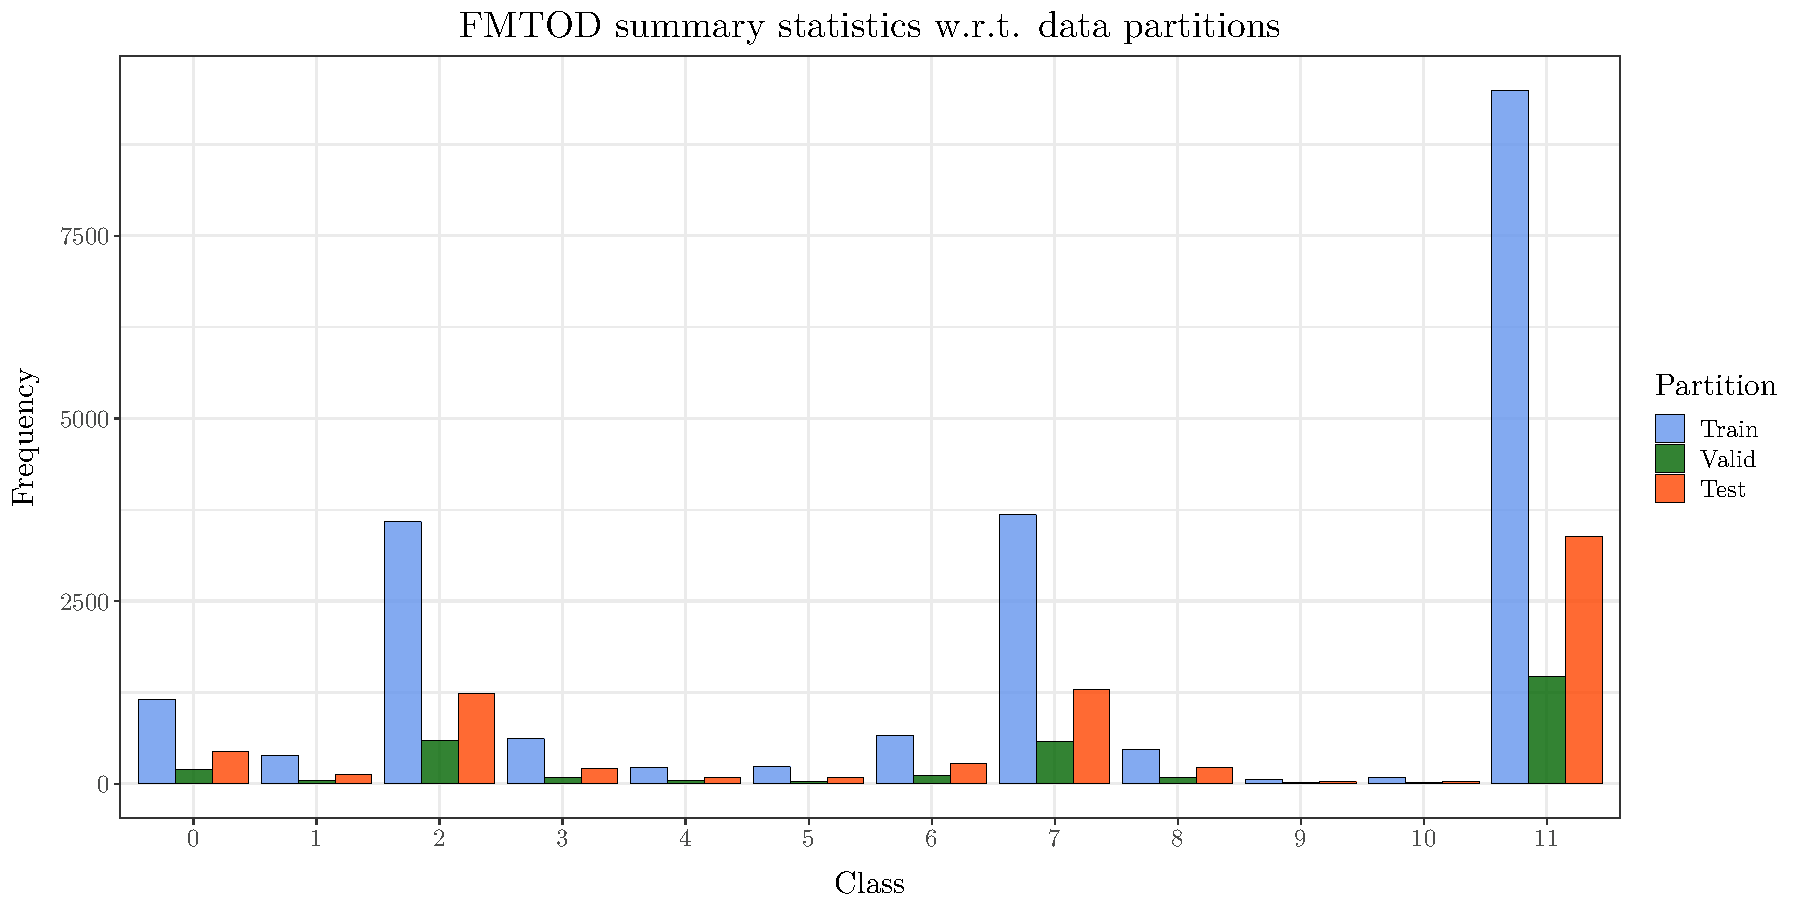
\includegraphics[width=14cm]{pdfs/generated/fmtod_summary_statistics.pdf}
  \caption{Frequency distribution of the preprocessed FMTOD data set by
    classes and partitions}
  \label{fig:fmtod}
\end{figure}

\begin{table}[t!]
  \centering
  \begin{tabular}{lllll}
    \toprule
    Class and description & Train & Validation & Test & $\Sigma$ \\
    \midrule
    0: \texttt{alarm/cancel\_alarm} & 1157 & 190 & 444 & 1791 \\
    1: \texttt{alarm/modify\_alarm} & 393 & 51 & 122 & 566 \\
    2: \texttt{alarm/set\_alarm} & 3584 & 596 & 1236 & 5416 \\
    3: \texttt{alarm/show\_alarms} & 619 & 83 & 212 & 914 \\
    4: \texttt{alarm/snooze\_alarm} & 228 & 49 & 89 & 366 \\
    5: \texttt{alarm/time\_left\_on\_alarm} & 233 & 30 & 81 & 344 \\
    6: \texttt{reminder/cancel\_reminder} & 662 & 114 & 284 & 1060 \\
    7: \texttt{reminder/set\_reminder} & 3681 & 581 & 1287 & 5549 \\
    8: \texttt{reminder/show\_reminders} & 474 & 82 & 217 & 773 \\
    9: \texttt{weather/check\_sunrise} & 63 & 13 & 25 & 101 \\
    10: \texttt{weather/check\_sunset} & 88 & 11 & 37 & 136 \\
    11: \texttt{weather/find} & 9490 & 1462 & 3386 & 14338 \\[5pt]
    \hline \hline \\[-10pt]
    $\Sigma$ & 20672 & 3262 & 7420 & 31354 \\
    \bottomrule
  \end{tabular}
  \caption{Frequency of the preprocessed FMTOD data set classes grouped by
    partitions; $\Sigma$ signifies the cumulative frequency statistic}
  \label{tab:fmtod}
\end{table}

During the preprocessing phase, many data duplicates were encountered and
correspondingly removed. Some of these duplicates observed were already present
in the original FMTOD data set, with additional duplicates being created from
the initial lowercasing step. After preprocessing, we obtain a lowercased
variant of the FMTOD data set with strictly unique data partitions. In the next
section, we describe the summary statistics of the preprocessed FMTOD data set.

\begin{table}[t!]
  \centering
  \begin{threeparttable}
    \begin{tabular}{lll}
      \toprule
      Class and description & Utterance length$^{\dagger}$ & Example$^{\ddagger}$ \\
      \midrule
      0: \texttt{alarm/cancel\_alarm} & 5.6 $\pm$ 1.9 & cancel weekly alarm \\
      1: \texttt{alarm/modify\_alarm} & 7.1 $\pm$ 2.5 & change alarm time \\
      2: \texttt{alarm/set\_alarm} & 7.5 $\pm$ 2.5 & please set the new alarm \\
      3: \texttt{alarm/show\_alarms} & 6.9 $\pm$ 2.2 & check my alarms. \\
      4: \texttt{alarm/snooze\_alarm} & 6.1 $\pm$ 2.1 & pause alarm please \\
      5: \texttt{alarm/time\_left\_on\_alarm} & 8.6 $\pm$ 2.1  & minutes left on my alarm \\
      6: \texttt{reminder/cancel\_reminder} & 6.6 $\pm$ 2.2 & clear all reminders. \\
      7: \texttt{reminder/set\_reminder} & 8.9 $\pm$ 2.5 & birthday reminders \\
      8: \texttt{reminder/show\_reminders} & 6.8 $\pm$ 2.2 & list all reminders \\
      9: \texttt{weather/check\_sunrise} & 6.7 $\pm$ 1.7 & when is sunrise \\
      10: \texttt{weather/check\_sunset} & 6.7 $\pm$ 1.7 & when is dusk \\
      11: \texttt{weather/find} & 7.8 $\pm$ 2.3 & jacket needed? \\[5pt]
      \hline \hline \\[-10pt]
      $\mu$ & 7.7 $\pm$ 2.5 & \textemdash \\
      \bottomrule
    \end{tabular}
    \begin{tablenotes}[flushleft]
      \footnotesize
      \item $^{\dagger}$Summary statistics follow the mean $\pm$
      standard-deviation format
      \item $^{\ddagger}$Short and simple examples were chosen for brevity and
      formatting purposes
    \end{tablenotes}
  \end{threeparttable}
  \caption{Utterance length summary statistics and examples for the preprocessed
    FMTOD data set; $\mu$ signifies the cumulative summary statistic}
  \label{tab:fmtod_examples}
\end{table}

\begin{table}[t!]
  \centering \def\arraystretch{1.3}
  \begin{tabular}{L{0.27\linewidth} L{0.45\linewidth} l}
    \toprule
    Study & Summary & Accuracy \\
    \midrule
    \citet{schuster-etal-2019-cross-lingual} & BiLSTM jointly trained on both the slot filling and intent classification tasks & 99.1$\%$ \\
    \citet{zhang2019joint} & BERT along with various decoders jointly fine-tuned on both the slot filling and intent classification tasks & 96.6--98.9$\%$ \\
    \citet{zhang-etal-2020-intent} & RoBERTa and XLM-RoBERTa fine-tuned on the English language and multilingual intent classification tasks along with WikiHow pre-training & 99.3--99.5$\%$ \\
    \bottomrule
  \end{tabular}
  \caption{Studies that addressed the FMTOD English language intent
    classification task along with their relevant summaries and accuracy
    ranges}
  \label{tab:fmtod_results}
\end{table}

\subsection{Summary statistics}

\label{section:fmtod_summary}

In regards to summary statistics of the preprocessed FMTOD data set, Figure
\ref{fig:fmtod} provides a visualization of the frequency distribution in the
data set grouped by classes and partitions; while Table \ref{tab:fmtod} shows
the same summary statistics in a tabular form with explicit frequencies. Based
on the summary statistics, we can observe that the preprocessed FMTOD data set
is significantly imbalanced with $\sim$45$\%$ of samples falling into Class 11
alone. We take this observation into consideration in later sections and apply
fixes to mitigate this data imbalance. In addition, we observe from Table
\ref{tab:fmtod_examples} that input utterances in the preprocessed FMTOD data
set are generally short; with a mean input utterance length of 7.7 and a
standard deviation of 2.5 tokens. Utterance length summary statistics were
computed with the assistance of NLTK's default \texttt{Treebank} word tokenizer
\citep{bird-loper-2004-nltk}.

\subsection{Performance range}

\label{section:fmtod_performance}

Several recent studies have addressed the FMTOD English language intent
classification task using a variety of deep neural networks such as BiLSTMs and
large language models such as XLM-RoBERTa
\citep{schuster-etal-2019-cross-lingual,zhang2019joint,zhang-etal-2020-intent}.
Table \ref{tab:fmtod_results} summarizes these studies along with their reported
accuracy scores on the FMTOD English language intent classification task. Based
on the presented results, we can observe that the competitive accuracy range for
the FMTOD English language intent classification task is 96.6-99.5$\%$.

\section{SoPa++}

We now introduce the main contribution of this thesis: the SoPa++ model.
Etymologically, SoPa++ derives its name from the variable increment operator
\texttt{"++"} used in programming languages such as C and Java. In essence, the
name SoPa++ signifies an improvement or major modification to the SoPa model.
Some of the major modifications from SoPa to SoPa++ include the utility of
strict linear-chain WFA-$\omega$'s over linear-chain WFAs, replacement of the
MLP in SoPa with quantized and transparent hidden layers and the introduction of
a new explanations by simplification post-hoc explainability technique which
leverages on the aforementioned modifications in SoPa++'s neural architecture.

\subsection{Strict linear-chain WFA-$\omega$'s}

As mentioned in Section \ref{section:sopa}, \citet{schwartz2018sopa} constructed
the SoPa model with an ensemble of linear-chain WFAs which permitted both
$\epsilon$ and self-loop transitions. As noted in Section \ref{section:sopa_cg},
$\epsilon$ and self-loop transitions are useful constructs in abstracting WFAs
and allowing them to consume variable length strings. However, based on
experimentation during our development phase; we observed a key concern that the
highest scoring substrings in the linear-chain WFAs in SoPa tended to have a
large variation of string lengths due to the effect of both
$\epsilon$-transitions and self-loops. We believe that this reduces the impact
of SoPa's explainability methods due to a lack of consistency in the lengths
of highest scoring paths and substrings. As a result, the first change we decided
for was to remove both $\epsilon$ and self-loop transitions in constituent WFAs
or patterns. With this change, we could at least ensure that each WFA would
always consume strings of fixed lengths.

However, consuming strings of fixed lengths could also be seen as a form of
overfitting in the model; since a model could simply memorize short strings or
phrases and would not necessarily incorporate any form of generalization. To
address this concern, we include a wildcard transition which we define here as a
$\omega$-transition. Allowing for such a transition was only natural since
wildcards are already crucial parts of regular expressions; which as we
mentioned are equivalent to FAs. To provide formalisms for this modification, we
provide the following definition for a WFA-$\omega$.

\begin{definition}[Weighted finite-state automaton-$\omega$]
  \label{def:wfa_w}
  A weighted finite-state automaton-$\omega$ over a semiring $\mathbb{K}$ is a
  5-tuple $\mathcal{A} = \langle \Sigma, \mathcal{Q}, \bm{\Gamma}, \bm{\lambda}, \bm{\rho}
  \rangle$, with:

  \begin{itemize}
  \itemsep0em
    \item[--] a finite input alphabet $\Sigma$;
    \item[--] a finite state set $\mathcal{Q}$;
    \item[--] transition matrix $\bm{\Gamma}: \mathcal{Q} \times \mathcal{Q} \times (\Sigma \cup \{\omega\}) \rightarrow \mathbb{K}$;
    \item[--] initial vector $\bm{\lambda}: \mathcal{Q} \rightarrow \mathbb{K}$;
    \item[--] and final vector $\bm{\rho}: \mathcal{Q} \rightarrow \mathbb{K}$.
  \end{itemize}

  \begin{remark}
    An $\omega$ transition is equivalent to a wildcard transition, which
    consumes an arbitrary token input and moves to the next state
  \end{remark}

  \begin{remark}
    Besides the inclusion of the $\omega$-transition and removal of the
    $\epsilon$-transition, a WFA-$\omega$ has all of the same characteristics
    as the WFA defined in Definition \ref{def:wfa}.
  \end{remark}
\end{definition}

Comparing with the linear-chain WFAs used in \citet{schwartz2018sopa} as per
Section \ref{section:sopa_lc_wfa}, our \textit{strict} linear-chain WFA-$\omega$
is similarly alloted a sequence of $|\mathcal{Q}|$ states. However, each state
$i$ in the linear-chain WFA-$\omega$ only has two possible outgoing transitions;
namely a \textbf{$\bm{\omega}$-transition} which consumes an arbitrary input
token and transitions to state $i+1$ and a \textbf{main-path transition} which
consumes a specific token and transitions to state $i+1$. Because of the
elimination of self-loop transitions, we refer to our linear-chain WFA-$\omega$
as strict linear-chain WFA-$\omega$ as per Remark
\ref{rmk:strict_linear_chain}. Similar to \citet{schwartz2018sopa}, we utilize
only the max-sum and max-product semirings in our strict linear-chain
WFA-$\omega$'s.

\begin{figure}[t!]
  \centering
  \includegraphics[width=14cm]{pdfs/generated/w_nfa_linear_chain/main.pdf}
  \caption{Visualization of a strict linear-chain NFA with
    $\omega$ (blue) and main-path (black) transitions}
  \label{fig:omega_fa}
\end{figure}

Next, we provide a mathematical formulation of the modified transition matrix
$\bm{\Gamma}$ in our strict linear-chain WFA-$\omega$. Here, $\bm{\Gamma}(x)$ represents a
$|Q|\times|Q|$ matrix containing transition scores when consuming an input token
$x$. $[\bm{\Gamma}(x)]_{i,j}$ corresponds to the cell value in $\bm{\Gamma}(x)$ for row
$i$ and column $j$ and represents the transition score when consuming token $x$
and transitioning from state $i$ to $j$.

\begin{equation}
  \label{eq:spp_transition_matrix_main}
  [\bm{\Gamma}(x)]_{i,j} =
  \begin{cases}
    \bm{w}_i \cdot \bm{v}_x + b_i  & \text{if } j = i + 1 \text{ (main-path transition),} \\
    \bar{0} & \text{otherwise.}
  \end{cases}
\end{equation}

Here, $\bm{w}_i$ and $b_i$ are learnable vectors and scalar biases
parameterizing transitions out of state $i$ to state $i+1$. $\bm{v}_x$
represents the word embedding for token $x$ and $\bar{0}$ represents the zero
value in the semiring used as per Definition \ref{def:semiring}. Similarly,
$\omega$-transitions are parameterized with the following representation in
$\bm{\Gamma}$:

\begin{equation}
  \label{eq:spp_transition_matrix_omega}
  [\bm{\Gamma}(\omega)]_{i,j} =
  \begin{cases}
    c_i  & \text{if } j = i + 1 \text{ ($\omega$-transition)} \\
    \bar{0} & \text{otherwise.}
  \end{cases}
\end{equation}

Here, $c_i$ represents a learnable scalar bias for $\omega$-transitions out of
state $i$ to state $i+1$. Finally as per \citet{schwartz2018sopa}, we fix the
initial vector $\bm{\lambda} = [\bar{1}, \bar{0}, \ldots, \bar{0}]$ and the final
vector $\bm{\rho} = [\bar{0}, \bar{0}, \ldots, \bar{1}]$, where $\bar{1}$ and
$\bar{0}$ represent the one and zero values specified in the semiring as per
Definition \ref{def:semiring}. The time-complexity of the Viterbi algorithm to
compute the string score for our linear-chain WFA-$\omega$'s is
$O(|Q||\bm{x}|)$, where $|\mathcal{Q}|$ refers to the number of states and
$|\bm{x}|$ refers to the length of the input string.

Ultimately, the introduction of a strict linear-chain WFA-$\omega$ allows us to
attain fixed string length consumption with an added layer of generalization
because of the introduction of wildcards. An example of a strict linear-chain
NFA extracted from a strict linear-chain WFA-$\omega$ is shown in Figure
\ref{fig:omega_fa}. Interestingly, we can observe that this NFA corresponds to
the Perl-compatible regular expression \texttt{``what a (great|entertaining)
  [\^{}\textbackslash\textbackslash s]+ !''}, where
\texttt{[\^{}\textbackslash\textbackslash s]+} refers to any set of consecutive
characters which are not separated by a space character. We can therefore infer
that a $\omega$-transition in a FA corresponds to the
\texttt{[\^{}\textbackslash\textbackslash s]+} regular expression term.

\begin{algorithm}[t!]
  \small
  \caption{Strict linear-chain WFA-$\omega$ document score$^*$}
  \label{algo:lc_wfa_w_document_score}
  \begin{algorithmic}[1]
    \Require{Strict linear-chain WFA-$\omega$ (denoted as $\mathcal{A}$) and document $\bm{y}$}
    \Ensure{Document score $s_{\text{doc}}(\bm{y})$}
    \Statex
    \Function{docscore}{$\mathcal{A}, \bm{y}$}
    \State $\bm{h}_0 \gets \big[\bar{1}, -\infty, \ldots, -\infty\big]$ \Comment{Create
      initial hidden state vector $\bm{h}_0: \mathcal{Q} \rightarrow \mathbb{K}$}
    \For{$i \gets 1,2,\ldots,\bm{|y|}$} \Comment{Sequentially iterate over each
      token $y_i \in \bm{y}$}
    \State $\bm{m} \gets \big[[\bm{\Gamma}(y_i)]_{1,2}, [\bm{\Gamma}(y_i)]_{2,3}, \ldots,
    [\bm{\Gamma}(y_i)]_{|\mathcal{Q}|-1,|\mathcal{Q}|}\big]$ \Comment{Main-path scores for token $y_i$}
    \State $\bm{\omega} \gets \big[[\bm{\Gamma}(\omega)]_{1,2}, [\bm{\Gamma}(\omega)]_{2,3}, \ldots,
    [\bm{\Gamma}(\omega)]_{|\mathcal{Q}|-1,|\mathcal{Q}|}\big]$
    \Comment{State-wise wildcard scores}
    \State $\bm{m'} \gets \bm{m} \otimes \bm{h}_{i-1}[:-1]$ \Comment{Path
      score with main-path transitions$^{\dagger}$}
    \State $\bm{\omega'} \gets \bm{\omega} \otimes \bm{h}_{i-1}[:-1]$ \Comment{Path
    score with $\omega$ transitions$^{\dagger}$}
    \State $\bm{h}_{i} \gets [\bar{1}] \mathbin\Vert \max(\bm{m'}, \bm{w'})$
    \Comment{Concatenate $\bar{1}$ to maximum of $\bm{m'}$ and $\bm{\omega'}$}    
    \EndFor
    \State $s_{\text{doc}}(\bm{y}) \gets  \max_{i \in 1,2,...,|\bm{y}|}
    \bm{h}_{i}[-1]$
    \Comment{Get maximum of hidden vector final states$^{\ddagger}$}
    \State \Return $s_{\text{doc}}(\bm{y})$
    \EndFunction
  \end{algorithmic}
  \algcomment{
    $^*$$\otimes$ and $\bar{1}$ are
    derived from max-based semirings where all semiring operations are element-wise \\
    $^{\dagger}\bm{h}_{i}[:-1]$ follows the Python indexing syntax
    and implies keeping all elements of $\bm{h}_{i}$ except the last \\
    $^{\ddagger}\bm{h}_{i}[-1]$ follows the Python indexing syntax and implies
    retrieving the last element of the vector $\bm{h}_{i}$
  }
\end{algorithm}

\subsection{Document score}

Similar to \citet{schwartz2018sopa}, SoPa++ was intended to compute scores for
entire documents and not just fixed-length strings using the strict linear-chain
WFA-$\omega$. To achieve this, we propose Algorithm
\ref{algo:lc_wfa_w_document_score} to compute the document score
$s_{\text{doc}}(\bm{y})$ for an arbitrary document $\bm{y}$. Here, we score all
consecutive substrings in a document $\bm{y}$ using either the max-sum or
max-product semirings assisted with the Viterbi algorithm. Following from this,
the document score $s_{\text{doc}}(\bm{y})$ for an arbitrary document $\bm{y}$
would reflect the highest path score which corresponds to a substring in
document $\bm{y}$.

\subsection{TauSTE}

In Section \ref{section:ste}, we described the concept of a STE in quantized
neural networks and explained how STEs function in both their forward and
backward passes. Furthermore, we provided a motivation as to why STEs and other
quantized activation functions are of interest; for example in relation to
computational savings linked to low-precision computing. In SoPa++, we make use
of a variant of the STE activation function which we define here as the Tau
Straight-through Estimator (TauSTE).

\begin{equation}
  \label{eq:tau_ste_forward}
  \text{TauSTE}(x)=
  \begin{cases}
    1 & x \in (\tau, +\infty) \\
    0 & x \in (-\infty, \tau]
  \end{cases}
\end{equation}

\begin{equation}
  \label{eq:tau_ste_backward}
  \text{TauSTE}'(x)=
  \begin{cases}
    1 & x \in  (1, +\infty) \\
    x & x \in [-1, 1] \\
    -1 & x \in (-\infty, -1) \\
  \end{cases}
\end{equation}

\begin{figure}[t!]
  \centering
  \includegraphics[width=14cm]{pdfs/generated/tau_ste_applied/main.pdf}
  \caption{Visualization of the TauSTE's forward and backward passes}
  \label{fig:tau_ste}
\end{figure}

A visualization of the TauSTE's forward and backward passes is shown in Figure
\ref{fig:tau_ste}. As we can see, there are two key changes from the vanilla STE
to the TauSTE. Firstly, the threshold for activation in the forward function is
now governed by a $\tau$-threshold such that $\tau \in \mathbb{R}$. This was
done to allow for some degree of freedom in deciding the activation threshold.
Secondly, the backward pass returns the identity function on $x \in [-1,1]$ and
remains fixed at -1 or +1 beyond these limits. This restriction was placed to
ensure that gradients do not blow up in size.

We chose to use the TauSTE because we believed it could prove useful for the
explainability purposes of our SoPa++ model. This is mainly because the TauSTE
(or even the STE) activation function simplifies continuous inputs into discrete
outputs; thereby reducing the information content of the signal it receives. In
later sections, we show how we capitalize on this reduction in signal
information in our SoPa++ model for our explanations by simplification post-hoc
explainability technique.

\subsection{Computational graph}

With the core modifications in the SoPa++ model explained, we now shift to
describing the computational graph or forward pass of the SoPa++ model by
referring to its various neural components. This description is linked to the
visualization of the computational graph of SoPa++ in Figure \ref{fig:spp_cg}.
Firstly, we utilize NLTK's default \texttt{Treebank} word tokenizer
\citep{bird-loper-2004-nltk} to conduct tokenization of input utterances into
word-level tokens. Next, we pad input utterances with special \texttt{[START]}
and \texttt{[END]} tokens at the start and end indices of the utterances to
signify the location where the utterance begins and ends. Finally, we utilize
GloVe 6B 300-dimensional uncased word-level embeddings
\citep{pennington2014glove} to project the input tokens to continuous numerical
spaces. 

\begin{figure}[t!]
  \centering
  \includegraphics[width=15cm]{pdfs/generated/spp_computational_graph/main.pdf}
  \caption{Visualization of the SoPa++ computational graph}
  \label{fig:spp_cg}
\end{figure}

Following this, we use our ensemble of $m \in \mathbb{N}$ strict linear-chain
WFA-$\omega$'s to traverse the input utterance and provide individual document
scores for this utterance; as prescribed by Algorithm
\ref{algo:lc_wfa_w_document_score}. When processing each input token, we monitor
the end states of each of the $m$ strict linear-chain WFA-$\omega$'s and
max-pool the score present in this state. In the edge case that an input string
was too short for the end state of a WFA-$\omega$ to register a non-$\bar{0}$
score, we simply discard this score in further analysis. This description so far
corresponds to the lower half of Figure \ref{fig:spp_cg}. After max-pooling
scores from all the $m$ strict linear-chain WFA-$\omega$'s, we then pass this
collection of pattern scores for further processing using SoPa++'s hidden neural
components; which can be seen in the upper portion of Figure \ref{fig:spp_cg}.
Firstly, we apply layer normalization \citep{ba2016layer} to all pattern scores
without any additional affine transformations. We omit the affine transformation
to not alter any of the pattern score information content and use layer
normalization as an expedient means of projecting the values of pattern scores
to a standard normal distribution. This normalization process guarantees that
pattern scores would be small in size and have a roughly even distribution of
positive and negative values around 0.

Layer normalization becomes very useful as we correspondingly encounter the
TauSTE layer. Here, the TauSTE layer maps all inputs which are strictly larger
than the $\tau \in \mathbb{R}$ threshsold to 1 and all others inputs to zero.
Naturally, the TauSTE layer is only useful when it is able to discriminate the
inputs by mapping some of them to 1 and some to 0, instead of always mapping all
inputs to either 1 or 0. Without layer normalization, the TauSTE layer would not
be able to perform its function since pattern scores tend to be mostly positive
with differing ranges. Layer normalization therefore helps to project these
variations of pattern scores to a uniform range; which ultimately allows the TauSTE
layer to discriminate inputs and produce diverse binary outputs.

A natural criticism of the TauSTE layer could be that it strongly limits the
flow of information in the SoPa++ model. While the binarization present in this
layer does indeed limit the rich flow of continuous numerical information, it is
still worth noting that this layer can preserve significant information given a
sufficiently large $m$ value, corresponding to the number of strict linear-chain
WFA-$\omega$ and TauSTE neurons. For example, if we allow for $m=40$ and therefore provide 40
WFA-$\omega$ and TauSTE neurons, we can have a total of
2$^{40}\approx1.1\times10^{12}$ binary state possibilities; which is slightly
greater than one trillion possible binary states. To provide some context to this
order of magnitude, the aforementioned number of possibilities is roughly equal
to estimated number of stars present in the Andromeda Galaxy
\citep{10.1093/mnras/stu879}. This would imply that despite the reduction in
information content on the TauSTE layer, there are still sufficient mappable
states available to learn various representations relevant to output classes;
given a large enough $m$ value or number of WFA-$\omega$.

After binarizing the hidden values in the TauSTE layer, we apply a simple linear
transformation to the TauSTE binary outputs to modify their dimensionality from
$m$ to $n \in \mathbb{N}$, where the $n$ represents the number of output
classes. We specifically chose a linear transformation layer over a MLP because
linear regressors are known to be transparent models
\citep{arrieta2020explainable} and this is a feature which ultimately assists us
in our explanations by simplification post-hoc explainability technique, which
we describe in greater detail in the next sections. Finally, we apply a softmax
function over the linear outputs to project them to probabalistic spaces and
then compute an \texttt{argmax} to extract the highest scoring index which represents the
predicted class. In the case of Figure \ref{fig:spp_cg}, the output class for
the input pre-processed utterance \texttt{``[START] 10 day weather forecast
  [END]''} is the \texttt{weather/find} class which corresponds to class index 11.

\subsection{Transparency}

\label{section:spp_transparency}

In regards to transparency, SoPa++ is a hybridized model consisting of RNN, CNN
and weighted finite-state neural components similar to that of SoPa. Following the
arguments of \citet{arrieta2020explainable} related to the black-box natures of
RNNs and CNNs, we can conclude that SoPa++ would correspondingly fall into the
black-box model category. Because of this classification, the SoPa++ model
would require post-hoc explainability techniques in order to explain its inner
mechanisms.

Reviewing the post-hoc explainability techniques offered by SoPa as per Section
\ref{section:sopa_post_hoc}, we would opine that a major limitation of these
techniques is that they do not fully capitalize on the rich theoretical
foundations offered by WFAs; such as their possible conversions to NFA and
ultimately regular expressions. In order to address this limitation, we propose
a new explanations by simplification post-hoc explainability technique for
simplifying a fully trained black-box SoPa++ model into a transparent regular
expression proxy model. We describe this new explanations by simplification
post-hoc explainability technique in the next section.

\section{RE proxy}

In this section, we describe the key processes required to convert a
fully trained black-box SoPa++ model into a transparent RE proxy model. These include
the introduction of a path-augmented document scoring algorithm and the creation
of the RE lookup layer. Next, we describe the computational graph or forward
pass of the RE proxy model. Finally, we provide some comments on
explainability-related aspects of the simplified RE proxy model and its
antecedent SoPa++ counterpart.

\subsection{Path-augmented document score}

\begin{algorithm}[t!]
  \small
  \caption{Strict linear-chain WFA-$\omega$ path-augmented document score$^*$}
  \label{algo:lc_wfa_w_document_score_trace}
  \begin{algorithmic}[1]
    \Require{Strict linear-chain WFA-$\omega$ (denoted as $\mathcal{A}$) and document $\bm{y}$}
    \Ensure{Document score $s_{\text{doc}}(\bm{y})$ and its corresponding path $\pi_{\text{doc}}(\bm{y})$}
    \Statex
    \Function{docscore\_path}{$\mathcal{A}, \bm{y}$}
    \State $\bm{h}_0 \gets \big[\bar{1}, -\infty, \ldots, -\infty\big]$ \Comment{Create
      initial hidden state vector $\bm{h}_0: \mathcal{Q} \rightarrow \mathbb{K}$}
    \For{$i \gets 1,2,\ldots,\bm{|y|}$} \Comment{Sequentially iterate over each
      token $y_i \in \bm{y}$}
    \State $\bm{m} \gets \big[[\bm{\Gamma}(y_i)]_{1,2}, [\bm{\Gamma}(y_i)]_{2,3}, \ldots,
    [\bm{\Gamma}(y_i)]_{|\mathcal{Q}|-1,|\mathcal{Q}|}\big]$ \Comment{Main-path scores for token $y_i$}
    \State $\bm{\omega} \gets \big[[\bm{\Gamma}(\omega)]_{1,2}, [\bm{\Gamma}(\omega)]_{2,3}, \ldots,
    [\bm{\Gamma}(\omega)]_{|\mathcal{Q}|-1,|\mathcal{Q}|}\big]$
    \Comment{State-wise wildcard scores}
    \State $\bm{m'} \gets \bm{m} \otimes \bm{h}_{i-1}[:-1]$ \Comment{Path
      score with main-path transitions$^{\dagger}$}
    \State $\bm{\omega'} \gets \bm{\omega} \otimes \bm{h}_{i-1}[:-1]$ \Comment{Path
    score with $\omega$ transitions$^{\dagger}$}
    \State $\bm{h}_{i} \gets [\bar{1}] \mathbin\Vert \max(\bm{m'}, \bm{w'})$
    \Comment{Concatenate $\bar{1}$ to maximum of $\bm{m'}$ and $\bm{\omega'}$}
    \State $\pi_i \gets \text{trace}(h_i[-1])$
    \Comment{Back-trace path $\pi_i$ corresponding to $h_i[-1]^{\ddagger}$}
    \EndFor
    \State $j \gets \argmax_{i \in 1,2,...,|\bm{y}|}
    \bm{h}_{i}[-1]$
    \Comment{Get index of final states' maximum$^{\ddagger}$}
    \State $s_{\text{doc}}(\bm{y}) \gets \bm{h}_{j}[-1]$
    \Comment{Get maximum final state value$^{\ddagger}$}
    \State $\pi_{\text{doc}}(\bm{y}) \gets \pi_j$
    \Comment{Get path of maximum final state value}
    \State \Return $[s_{\text{doc}}(\bm{y}), \pi_{\text{doc}}(\bm{y})]$
    \EndFunction
  \end{algorithmic}
  \algcomment{
    $^*$$\otimes$ and $\bar{1}$ are
    derived from max-based semirings where all semiring operations are element-wise \\
    $^{\dagger}\bm{h}_{i}[:-1]$ follows the Python indexing syntax
    and implies keeping all elements of $\bm{h}_{i}$ except the last \\
    $^{\ddagger}\bm{h}_{i}[-1]$ follows the Python indexing syntax and implies
    retrieving the last element of the vector $\bm{h}_{i}$
  }
\end{algorithm}

One major advantage of the Viterbi algorithm, as per Definition
\ref{def:string_score}, is its ability to return the highest path score which
can ultimately allow for attribution to a certain path and substring in a
document. In order to simplify SoPa++ into a RE proxy model, we first need to
modify our document scoring algorithm to not only return the document score
$s_{\text{doc}}(\bm{y})$ but also its corresponding path
$\pi_{\text{doc}}(\bm{y})$. This process is described as a path-augmented
document score in Algorithm \ref{algo:lc_wfa_w_document_score_trace}, where we
trace the exact path of each transition and return the best path in addition to
the highest path score. Similar to Algorithm \ref{algo:lc_wfa_w_document_score},
this algorithm has a time-complexity of $O(|Q||\bm{x}|)$, where
$|\mathcal{Q}|$ refers to the number of states in a strict linear-chain
WFA-$\omega$ and $|\bm{x}|$ refers to the length of the input string. It is also
worth mentioning that the highest scoring path returned ultimately reflects a set of
transitions in the form of a strict linear-chain NFA; which can correspondingly
be transformed into a regular expression. Therefore, it can be inferred that
Algorithm \ref{algo:lc_wfa_w_document_score_trace} returns the best scoring
regular expression corresponding to a certain strict linear-chain WFA-$\omega$.

\subsection{RE lookup layer}

The next step in simplifying a fully-trained SoPa++ to a RE proxy model is the
extraction of a RE lookup layer. To motivate this process, we shortly revert to
the SoPa++ computational graph in Figure \ref{fig:spp_cg}. The TauSTE layer
filters input signals from normalized pattern scores and provides +1 outputs for
normalized pattern scores which exceed the $\tau$-threshold. Since pattern
scores correspond to document scores and document scores can be augmented with
best paths and regular expressions as per Algorithm
\ref{algo:lc_wfa_w_document_score_trace}, we can assign the activation of each
TauSTE neuron for each input utterance with an "activating" regular expression.
By iterating over all our training data, we can collect many such "activating"
regular expressions which activate the various TauSTE neurons; such that each
TauSTE neuron $\bm{N_i}$ is assigned a set of "activating" regular expressions
\textbf{\{RE\}$_i$}. The collection of all regular expressions
$[\{\textbf{RE}\}_1, \ldots, \{\textbf{RE}\}_m]$ which activate $m$ TauSTE
neurons is known as the RE lookup layer. Overall, the RE lookup layer represents
a knowledge base of important regular expressions that cause the SoPa++ model to
make a weighted decision. This process of extracting the RE lookup layer from
the SoPa++ model is reflected in Algorithm \ref{algo:simplification_process}.

\begin{algorithm}[t!]
  \small
  \caption{Extracting RE lookup layer from SoPa++}
  \label{algo:simplification_process}
  \begin{algorithmic}[1]
    \Require{Trained SoPa++ model $\mathcal{S}$ and training data $[\bm{y}_1, \ldots, \bm{y}_t]$}
    \Ensure{RE lookup layer $[\{\textbf{RE}\}_1, \ldots, \{\textbf{RE}\}_m]$}
    \Statex
    \Function{extract\_lookup}{$\mathcal{S}, [\bm{y}_1, \ldots, \bm{y}_t]$}
    \State $[\{\textbf{RE}\}_1, \ldots, \{\textbf{RE}\}_m] \gets [\emptyset,
    \ldots, \emptyset]$
    \Comment{Initialize RE lookup layer}
    \For{$i \gets 1,2,\ldots,t$}
    \Comment{Loop over training data}
    \For{$j \gets 1,2,\ldots,m$}
    \Comment{Loop over WFA-$\omega$'s in $\mathcal{S}$}
    \State $\mathcal{A}_j \gets \text{get\_WFA}(\mathcal{S}, j)$
    \Comment{Get WFA-$\omega$ by index}
    \State $s^j_{\text{doc}}(\bm{y}_i), \pi^j_{\text{doc}}(\bm{y}_i) \gets
    {\small\textsc{docscore\_path}}(\mathcal{A}_j, \bm{y}_i)$
    \If{TauSTE$(s^j_{\text{doc}}(\bm{y}_i)) == 1$}
    \State $\{\textbf{RE}\}_j \gets \{\textbf{RE}\}_j \cup
    \pi^j_{\text{doc}}(\bm{y}_i)$
    \Comment{Save $\pi^j_{\text{doc}}(\bm{y}_i)$ if it activates TauSTE} 
    \EndIf
    \EndFor
    \EndFor
    \State \Return $\text{compress}([\{\textbf{RE}\}_1, \ldots, \{\textbf{RE}\}_m])$
    \Comment{Compress RE lookup layer} 
    \EndFunction
  \end{algorithmic}
\end{algorithm}

This leads us to several interesting conclusions. Firstly, we observe here that
the TauSTE layer is not only useful for reducing information complexity; but
also for attributing causal links to SoPa++'s decision-making. In this case,
the causal links are the "activating" regular expressions returned by the
strict-linear chain WFA-$\omega$ when computing the path-augmented document
score. Next, we can also observe the effect of the $\tau$-threshold on the RE
lookup layer. If the $\tau$-threshold is low, we effectively allow more TauSTE
neurons to be activated and therefore allow more regular expressions from the
strict linear-chain WFA-$\omega$ to be saved in the RE lookup layer.
Contrastingly, if the $\tau$-threshold is high; we allow fewer TauSTE neurons to
be activated and therefore allow fewer regular expressions to be saved in the RE
lookup layer. It is not necessarily clear whether small or large
$\tau$-thresholds are better for performance; but a larger $\tau$-threshold and
therefore smaller RE lookup layer could be beneficial for explainability
purposes since the RE knowledge base would be smaller and possbily easier
to comprehend for a human. 

\begin{figure}[t!]
  \centering
  \includegraphics[width=15cm]{pdfs/generated/regex_computational_graph/main.pdf}
  \caption{Visualization of the RE proxy computational graph}
  \label{fig:regex_cg}
\end{figure}

\subsection{Assembling RE proxy}

The final step in simplifying a fully-trained SoPa++ model into a RE proxy model
is to assemble the RE proxy model using the RE lookup and SoPa++ linear layers.
Specifically, for a given SoPa++ model; we firstly extract the RE lookup layer.
Then, we combine the RE lookup layer and the SoPa++ linear layer in order to
create the RE proxy model. A visualization of this is shown in Figure
\ref{fig:regex_cg} and we can observe how the RE lookup layer essentially
replaces most of the lower neural components of the SoPa++ model up until the
TauSTE layer. The resulting RE proxy should ideally be a good approximator
of the SoPa++ model; with the exact degree of approximation being an empirical
matter. Given this process of assembly, it is important to note that each SoPa++
model allows for exactly one RE proxy model that can be assembled. Therefore, SoPa++
and RE proxy models occur in model-pairs.

One major limitation of the RE proxy model is in its RE lookup layer. Since the
RE lookup layer is essentially a memorized knowledge base, it could contribute
to overfitting on the training data and result in a RE proxy model that is not
representative of the SoPa++ model on unseen data. While this limitation could
theoretically be offset by the presence of sufficient variable-length regular
expression samples with wildcards, it would ultimately boil down to an empirical
investigation to quantify how similar the RE proxy model is to its antecedent
SoPa++ model.

\subsection{Computational graph}

We now provide a description of the computational graph or forward pass of the
assembled RE proxy model with reference to Figure \ref{fig:regex_cg}. Similar to
the computational graph of SoPa++, we process our input text sequentially.
However, instead of using token embeddings and neural network components; we
pass our input utterance through our RE lookup layer which conducts substring
matches over all sets of regular expressions in $[\{\textbf{RE}\}_1, \ldots,
\{\textbf{RE}\}_m]$. If any regular expression set $\{\textbf{RE}\}_i$ matches
the input utterance, the index of this RE set if given a value of 1. If no
regular expression in the set matches, the index of this RE set is given a value
of 0. These values are assembled into a binary vector that mimics the outputs of
the TauSTE layer in the antecedent SoPa++ model. This binary vector is then
passed to the linear regression layer; which transforms the binary vector back
into continuous space with the appropriate dimensionality. Following softmax and
argmax operations, we arrive at our predicted output class. It is worth
mentioning that while the execution of the SoPa++ forward pass can be
accelerated due to tensor-based parallelization with hardware acceleration on a
Graphics Processing Unit (GPU), the forward pass of the RE proxy model is
significantly slower due to our unoptimized single-threaded RE lookup process.

\subsection{Transparency}

\label{sec:re_transparency}

So far, we have described the process of simplifying a fully-trained black-box
SoPa++ model into a RE proxy model. We now investigate the RE proxy model and
comment on its degree of transparency. In essence, a RE proxy model consists of
a RE lookup layer followed by a linear regressor. The RE lookup layer can be
seen as a rules-based learner component where inputs are processed via clear and
interpretable RE matching rules to produce outputs. Since both rules-based
learners and linear regressors can be considered as transparent models as per
\citet[Page 7, Section 3]{arrieta2020explainable}, we could theoretically
classify the RE proxy model as a transparent model. However, it is important to
note that this is only a theoretical argument which could be disproven in given
practical cases. For example as per \citet[Page 9, Table
2]{arrieta2020explainable}, rules-based learners and linear regressors could be
viewed as black-box models if they require the handling of an incomprehensible
number of rules or input features. This could also be the case for the RE proxy
model depending most importantly on the size of the RE lookup layer.

\subsection{Explainability}

We now provide additional comments on the explanations by simplification
post-hoc explainability technique to simplify a fully-trained black-box SoPa++
model into a transparent RE proxy model. Firstly, we would assign the target
audience of this explainability technique as expert-users compared to the
inferred target audience of average end-users for the SoPa model. We designate
expert-users as our target audience mainly because the process of constructing
and understanding the RE proxy model is not as straightforward as the local
explanations and feature relevance techniques in SoPa as per Section
\ref{section:sopa_post_hoc}.

Next, we evaluate the quality of explanations offered by using the explanations
by simplification technique using the three guidelines offered in Section
\ref{section:xai_metrics}. Regarding the constrictive quality, it is likely that
the RE proxy model meets this criterion since the linear layer contains easily
interpretable weights which could explain which matched regular expressions were
scored higher or lower. Regarding causal links, it is likely that the RE proxy
model meets this criterion since the RE lookup layer matches fixed REs whose
binary matching scores are then clearly propagated from the start to the end of
the model. Therefore, a decision occurring at the end of the model could be
easily causally attributed to the start of the model. Regarding the selective
quality, it is possible that the RE proxy model meets this criterion since the
linear weights applied to matched regular expressions can be easily ranked to
understand which were the most important causal links influencing the model's
decision.

\begin{table}[t!]
  \centering \def\arraystretch{1.3}
  \begin{tabular}{L{0.275\linewidth} L{0.3\linewidth} L{0.3\linewidth}}
    \toprule
    Characteristic & SoPa & SoPa++ \\
    \midrule
    Text casing & True-cased & Lower-cased \\ 
    Token embeddings & GloVe 840B 300-dimensions & GloVe 6B 300-dimensions \\
    WFAs & Linear-chain WFAs with $\epsilon$, self-loop and main-path transitions & Strict linear-chain WFA-$\omega$'s with $\omega$ and main-path transitions \\
    Hidden layers & Multi-layer perceptron after max-pooling & Layer normalization, TauSTE and linear transformation after max-pooling \\
    Post-hoc explainability technique(s) & Local explanations, feature relevance & Explanations by simplification \\
    \bottomrule
  \end{tabular}
  \caption{Summarized differences for SoPa vs. SoPa++}
  \label{tab:sopa_spp_comparison}
\end{table}

\section{Differences between SoPa and SoPa++}

To wrap up this current segment on the SoPa++ model, we summarize the key
differences between SoPa and SoPa++ as shown in Table
\ref{tab:sopa_spp_comparison}. The most significant modifications to SoPa++
include the modification of linear-chain WFAs to strict linear-chain
WFA-$\omega$'s, the replacement of the MLP with layer normalization, TauSTE and
linear layers and the significantly different explanations by simplification
post-hoc explainability technique to create RE proxy models. With the
construction of SoPa++ and its RE proxy models established, we now proceed to
describe the methodologies used to answer our three research questions.

\section{RQ1: Evaluating performance of SoPa++}

In this section, we describe the methodologies used to answer our first research
question regarding the competitive performance of the SoPa++ model on the FMTOD
data set. Specifically, we describe how we trained the SoPa++ model and
afterwards, how we proceeded to evaluate and compare its performance to other
studies.

\subsection{Training}

\label{section:spp_training}

First and foremost, we address the issue of data imbalance in the FMTOD data set
as mentioned in Section \ref{section:fmtod_summary}. For this, we chose a simple
but effective solution of upsampling all minority data classes such that they
would have the same frequency as the majority class. We chose this approach over
other approaches such as gradient-weighting since this is generally a model
agnostic and straightforward approach.

Returning to the computational graph of SoPa++ in Figure \ref{fig:spp_cg}, we
compute the cross-entropy loss using the softmax output and target one-hot
encoded classes. Since SoPa++ is in essence a deep neural network, we utilize
the well-studied gradient descent technique to train and update our SoPa++ model
with the objective of minimizing the aforementioned cross-entropy loss. To
facilitate this learning process, we utilize
PyTorch\footnote{https://pytorch.org/} to assist with gradient computations,
backward passes and parallelized tensor computations. We utilize the Adam
optimizer \citep{DBLP:journals/corr/KingmaB14} to stabilize the gradient descent
learning technique with $\beta_1=0.9$ and $\beta_2=0.999$. In terms of fixed
training hyperparameters, we utilize a learning rate of 0.001, a batch size of
256 input utterances and neuron/word dropout probabilities of 0.2. We only apply
neuron dropouts on the transition matrices of all the strict linear-chain
WFA-$\omega$'s in SoPa++. We furthermore apply batch sorting based on input
utterance lengths to ensure maximum efficiency when computing pattern/document
scores. Based on our own experiments, we observed more stable training with the
max-sum semiring compared to the max-product semiring. For simplicity, we
therefore only use the max-sum semiring in all of our WFA-$\omega$'s.

\begin{table}[t!]
  \centering
  \begin{tabular}{lll}
    \toprule
    Model & Pattern hyperparameter $P$ & Parameter count \\
    \midrule
    Small & \texttt{6-10\_5-10\_4-10\_3-10} & 1,260,292 \\
    Medium & \texttt{6-25\_5-25\_4-25\_3-25} & 1,351,612  \\
    Large & \texttt{6-50\_5-50\_4-50\_3-50} & 1,503,812 \\
    \bottomrule
  \end{tabular}
  \caption{Three different SoPa++ model sizes used during training with
    corresponding pattern hyperparameter $P$ and parameter counts}
  \label{tab:model_types}
\end{table}

To obtain some variation in our SoPa++ models, we decide to use a grid-search
technique while varying the patterns $P$ and $\tau$-threshold hyperparameters.
Our variations in the patterns hypereparameter $P$ result in three different
SoPa++ model sizes which we define as small, medium and large as per Table
\ref{tab:model_types}. Correspondingly, we vary the $\tau$-threshold
hyperparameter with the following five possible values: $\{0.00, 0.25, 0.50,
0.75, 1.00\}$. For each model configuration in our grid-search routine, we
repeat a model run ten times with different initial random seeds in order to
obtain a distribution of performances. In total, our grid-search routine
produces a total of $3\times5\times10=150$ model runs. Finally, we train all
models for a maximum of 50 epochs with 10 patience epochs for early stopping in
case of a performance plateau or worsening. To trigger early stopping in the
patience framework, we monitor the cross-entropy loss over the validation data
set. We run all SoPa++ training experiments on a single NVIDIA GeForce GTX 1080
Ti GPU for $\sim$24 hours.

\subsection{Evaluation}

Given fully trained SoPa++ models from the previous training step, we now
proceed to evaluate the performance of the SoPa++ models on the FMTOD data set's
test partition. We simply run the preprocessed FMTOD test partition through the
computational graph of the SoPa++ model and obtain the predicted classes. With
the predicted and target classes, we compute the accuracy of the SoPa++ models
and summarize these to obtain a distribution of performances over the random
seed iterations. Finally, we compare our mean accuracies with the accuracy range
of other recent papers on FMTOD as described in Section
\ref{section:fmtod_performance}. If the mean accuracy of our SoPa++ models
falls into the aforementioned competitive range, we can then conclude that our
SoPa++ model performs competitively with other recent studies.

\section{RQ2: Evaluating explanations by simplification}

\label{section:evaluate_explain}

We now move on to describe the methodologies pursued to answer our second
research question on evaluating the effectiveness of our explanations by
simplification post-hoc explainability method. As mentioned in Definition
\ref{def:explain_simplify}, the purpose of explanations by simplification is to
create a less complex proxy model which can both keep a similar performance
score and maximize its resemblance to the antecedent model. We already discussed
how the RE proxy derived from SoPa++ is likely to be a transparent model
compared to the black-box SoPa++ model; which already satisfies the important
criterion that the proxy model should be less complex.

To address the similarity of the performance scores of both SoPa++ and RE proxy
model pairs, we compute and compare the accuracy scores of model pairs on the
FMTOD data set's test partition since this represents previously unseen data for
both SoPa++ and its RE proxy model pair and could provide an unbiased
representation of the performances of both models. The final criterion for
effective explanations by simplification is to ensure maximum resemblance
between the antecedent and proxy models. In order to evaluate the degree of
resemblance, we propose computing the following two inner-model distance metrics
to quantify the distance between the SoPa++ and RE proxy model pairs. Naturally,
a smaller distance metric would symbolize greater resemblance between model pairs.

\subsection{Softmax distance norm}

One method of quantifying a distance between
the SoPa++ and RE proxy model pairs is to run both of them on the FMTOD test
data set and obtain the softmax scores on each sample. Next, we can find the
Euclidean norm of the difference of these two softmax vectors. A low softmax
Euclidean distance norm would imply that the softmax distributions are similar
and would imply, to a certain extent, that the models conducted similar
weightings of input features. This method is not a perfect indicator of
interpreting distances between models; but it is more refined in that it allows
us to analyze continuous vector differences. We provide a mathematical
formulation of the softmax distance norm $\delta_{\sigma}(\bm{y})$ below for a single
document $\bm{y}$ where $\sigma_{\mathcal{S}}$ and $\sigma_{\mathcal{R}}$ represent the
softmax vectors for the SoPa++ and RE proxy model on the given sample
respectively and $n$ represents the number of classes in the FMTOD data set:

\begin{equation}
  \delta_{\sigma}(\bm{y}) = \left\Vert \sigma_{\mathcal{S}}(\bm{y}) - \sigma_{\mathcal{R}}(\bm{y}) \right\Vert_{2} = \sqrt{\sum^n_{i=1} (\sigma_{\mathcal{S}_i}(\bm{y}) - \sigma_{\mathcal{R}_i}(\bm{y}))^2} 
\end{equation}

\subsection{Binary misalignment rate}

Another technique of measuring the
distance between the SoPa++ and RE proxy model would be to compare their
internal representations activated in the TauSTE binary layer. This can be
computed by calculating the 1-norm between the binary vectors and then
normalizing this norm by the dimensionality of this vector. The step of
normalization is necessary since we test models with different sizes and these
could have different binary vector lengths. This would provide a mean binary
misalignment rate $\delta_b(\bm{y})$ for a single document $\bm{y}$, where
$b_{\mathcal{S}}$ and $b_{\mathcal{R}}$ represent the TauSTE binary vectors for
the SoPa++ and RE proxy model respectively and $dim$ represents an operator that
retrieves the dimensionality of a vector space:

\begin{equation}
  \delta_b(\bm{y}) = \dfrac{\left\Vert b_{\mathcal{S}}(\bm{y}) - b_{\mathcal{R}}(\bm{y}) \right\Vert_{1}}{dim(b_{\mathcal{S}}(\bm{y}) - b_{\mathcal{R}}(\bm{y}))} = \dfrac{\sum^n_{i=1} |b_{\mathcal{S}_i}(\bm{y}) - b_{\mathcal{R}_i}(\bm{y})|}{{dim(b_{\mathcal{S}}(\bm{y}) - b_{\mathcal{R}}(\bm{y}))}}
\end{equation}

\section{RQ3: Interesting and relevant explanations}

In this section, we describe the methodologies utilized to answer our third
research question; particularly to show what interesting and relevant
explanations the SoPa++ model can provide on the FMTOD data set.

\subsection{Output neuron weights}

Since SoPa++ uses a linear regression layer to provide weights and biases
towards TauSTE outputs, we can analyze the weights of the linear regression
layer to probe into how the SoPa++ and its RE proxies distribute importances to
various binary features present in the TauSTE layer. This is a major advantage
of using a single additive layer such as the linear regression layer, compared
to using a MLP. To go about this, we simply perform a softmax operation over all
weights applied for each class in each TauSTE neuron; and then visualize these
to observe how SoPa++ and its RE proxies distribute feature importance.

\subsection{Regular expression lookup layer}

One major advantage of producing simpler RE proxy models is the presence of the
RE lookup layer. This RE lookup layer can be seen as an ontology or database of
REs that lead to activations in the TauSTE layer. As a result, the RE lookup
layer can be seen as an ontology of important regular expressions that aid
SoPa++ and its RE proxies in making decisions based on input utterances. We
analyze some of these REs juxtaposed next to their representative TauSTE neurons
to visualize which REs activate which neurons and what kinds of importances are
placed in said REs.

%%% Local Variables: 
%%% mode: latex
%%% TeX-master: "main"
%%% End: 